%---------------------------------------
% References
%---------------------------------------
\clearpage
\phantomsection
\addcontentsline{toc}{chapter}{References}
\bibliographystyle{plain}
\bibliography{references}

%---------------------------------------
% Appendices  (replaces everything after \appendix in backmatter.tex)
% Figures: copy every PNG of figures.zip into thesis_report/thesis/figures/
%---------------------------------------
\appendix

\chapter{Additional figures}
\label{app:figures}

\section{Data and explainer}

\begin{figure}[htbp]
\centering
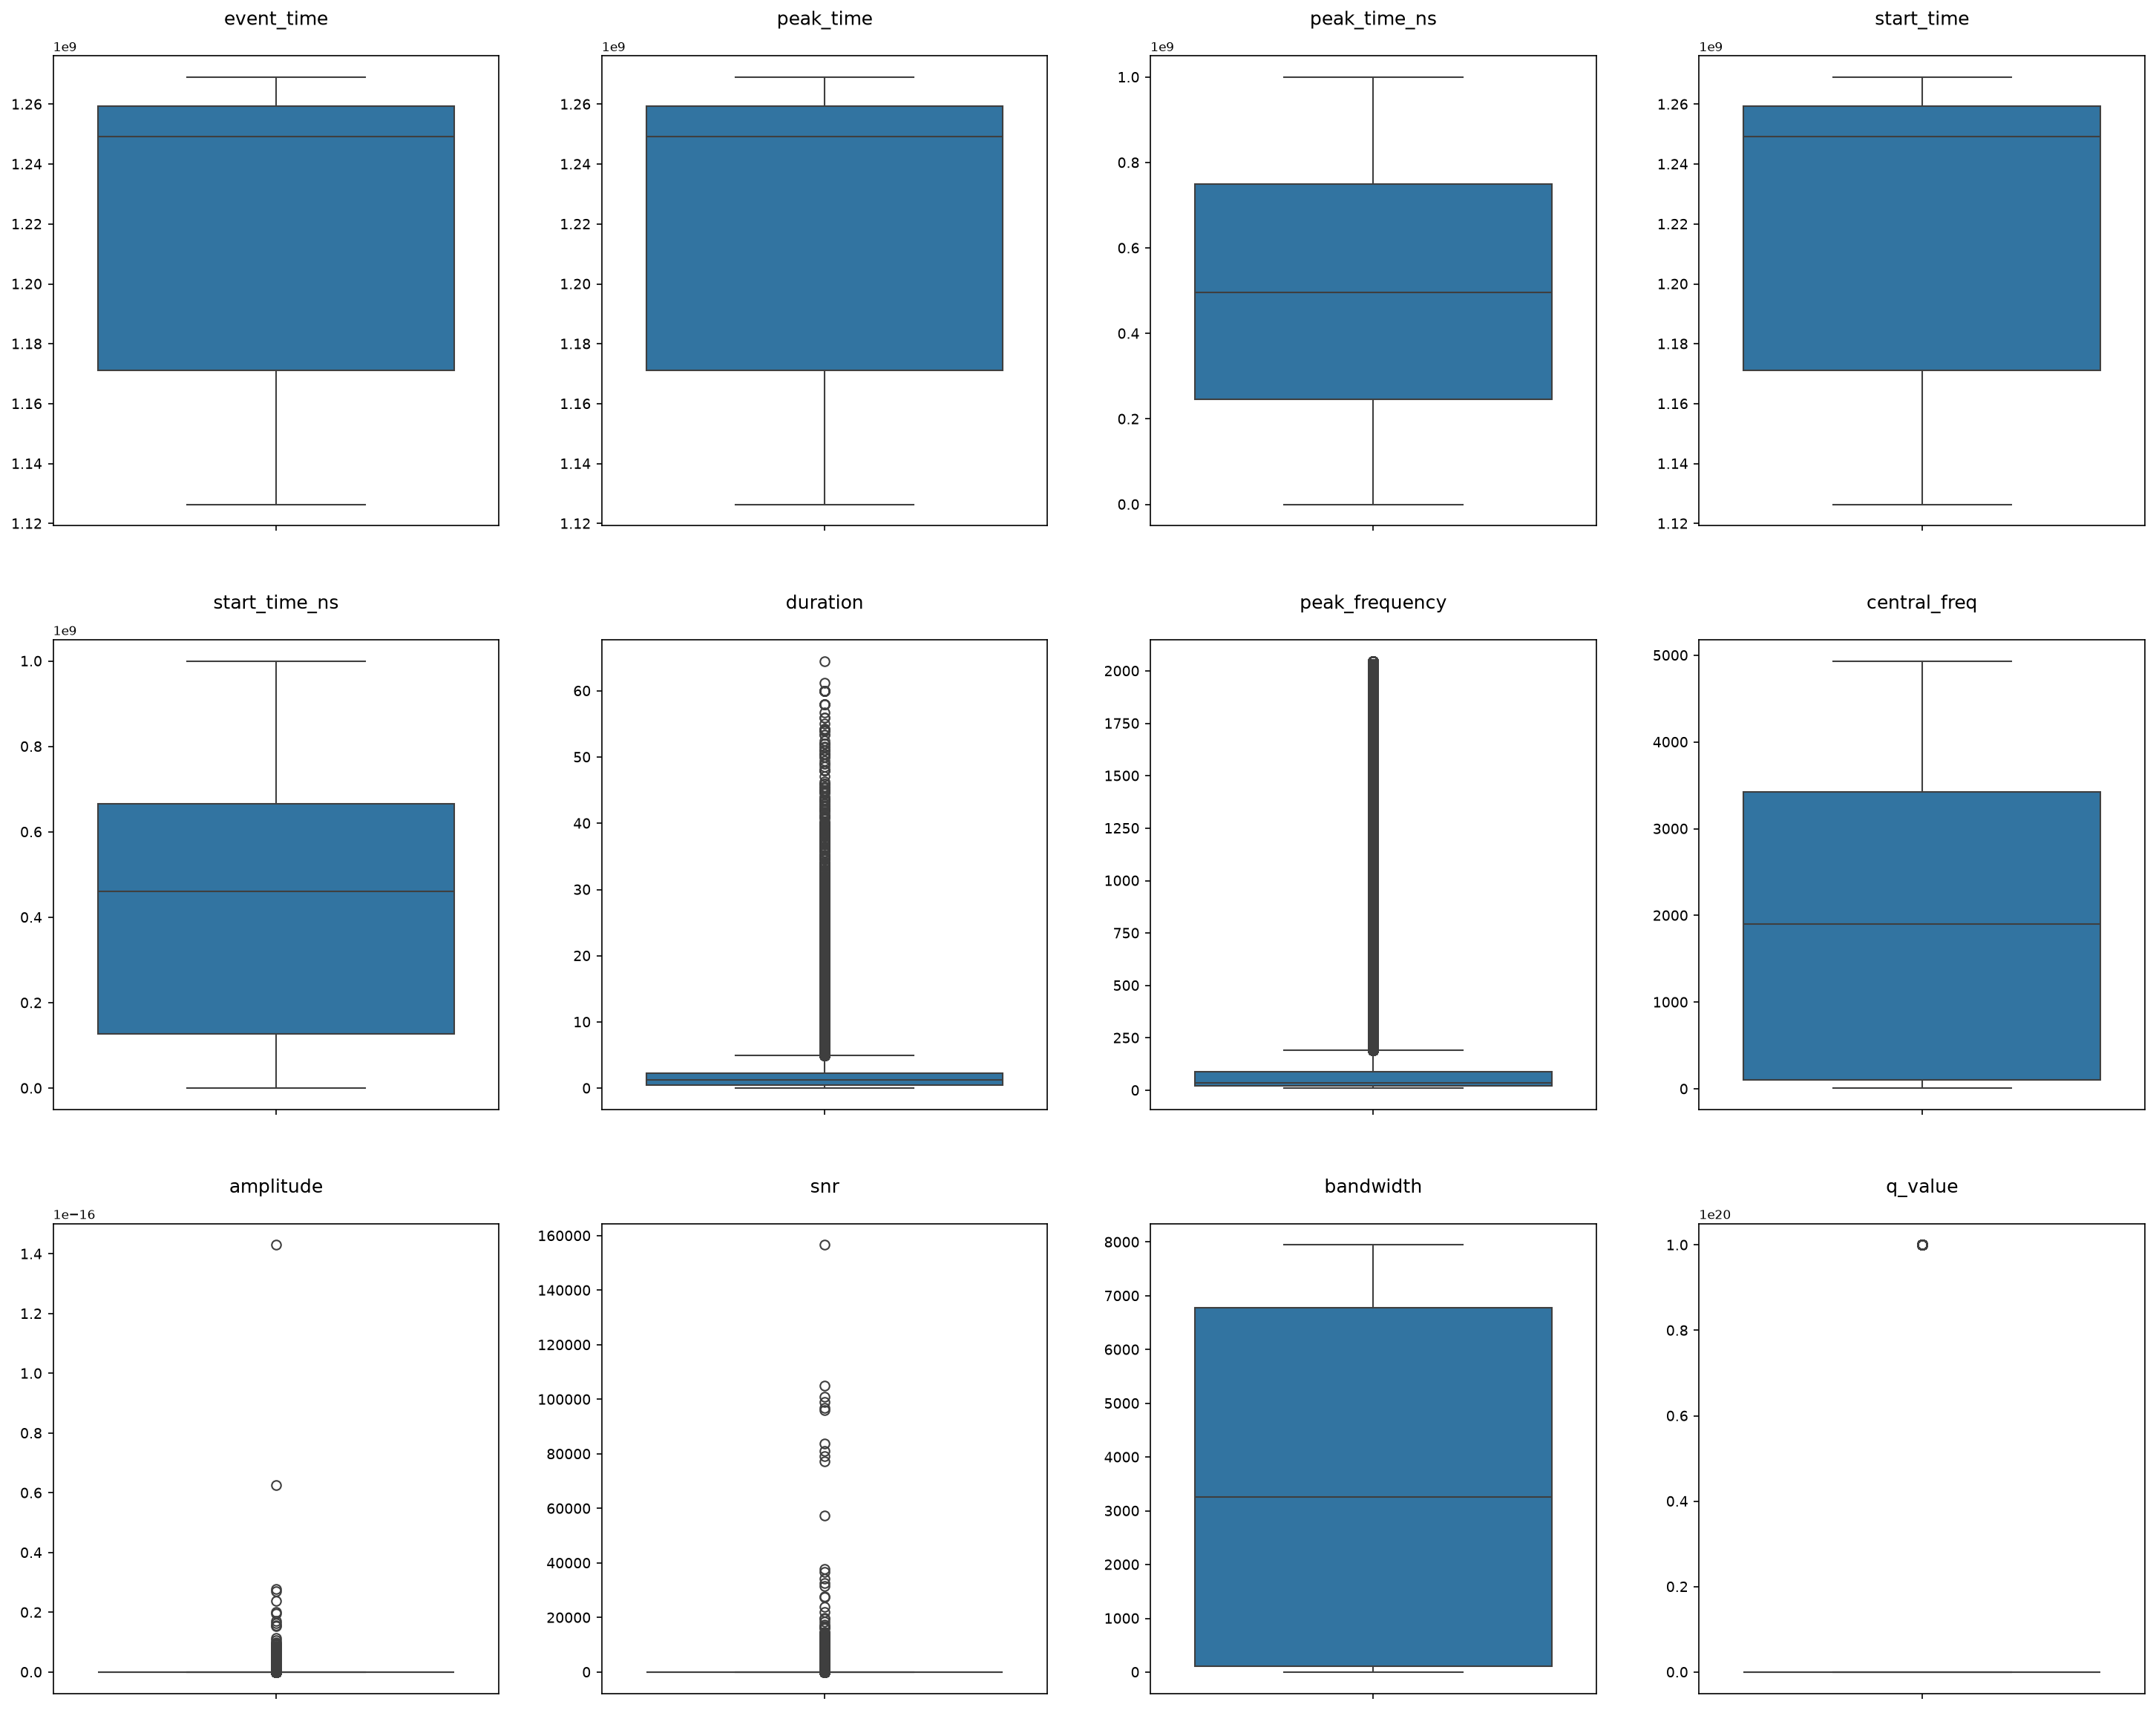
\includegraphics[width=\linewidth]{feature_boxplots.png}
\caption{Distributions of the twelve numerical Omicron descriptors over the full
release. The quality factor collapses to a sentinel value of order $10^{20}$;
amplitude and SNR are dominated by a long tail of outliers.}
\label{fig:boxplots}
\end{figure}

\begin{figure}[htbp]
\centering
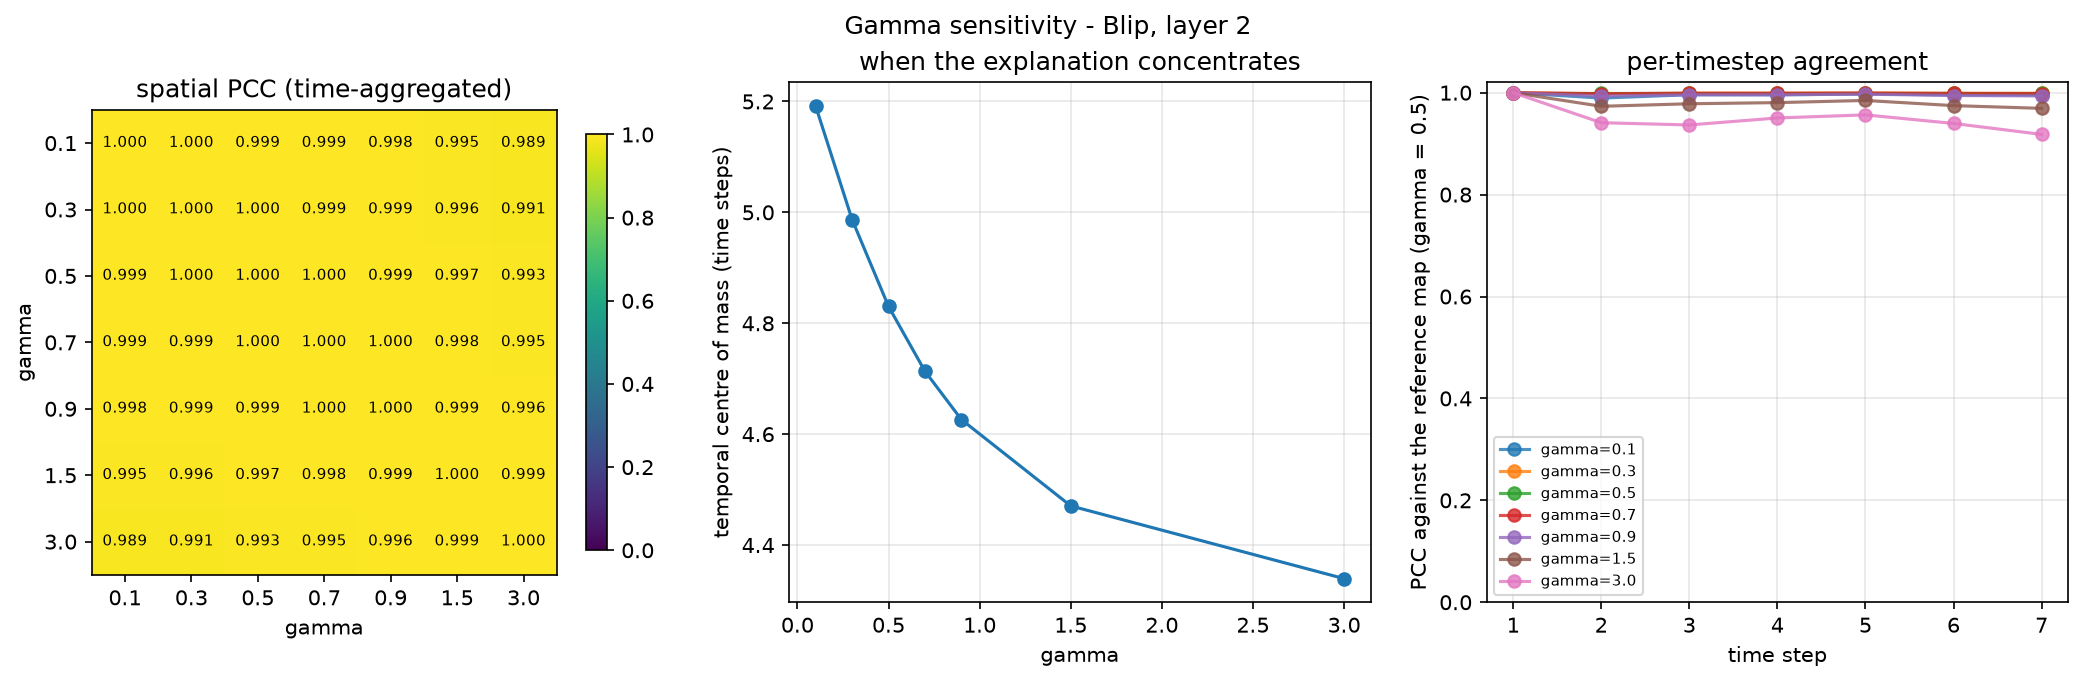
\includegraphics[width=\linewidth]{gamma_Blip.png}\\[0.5em]
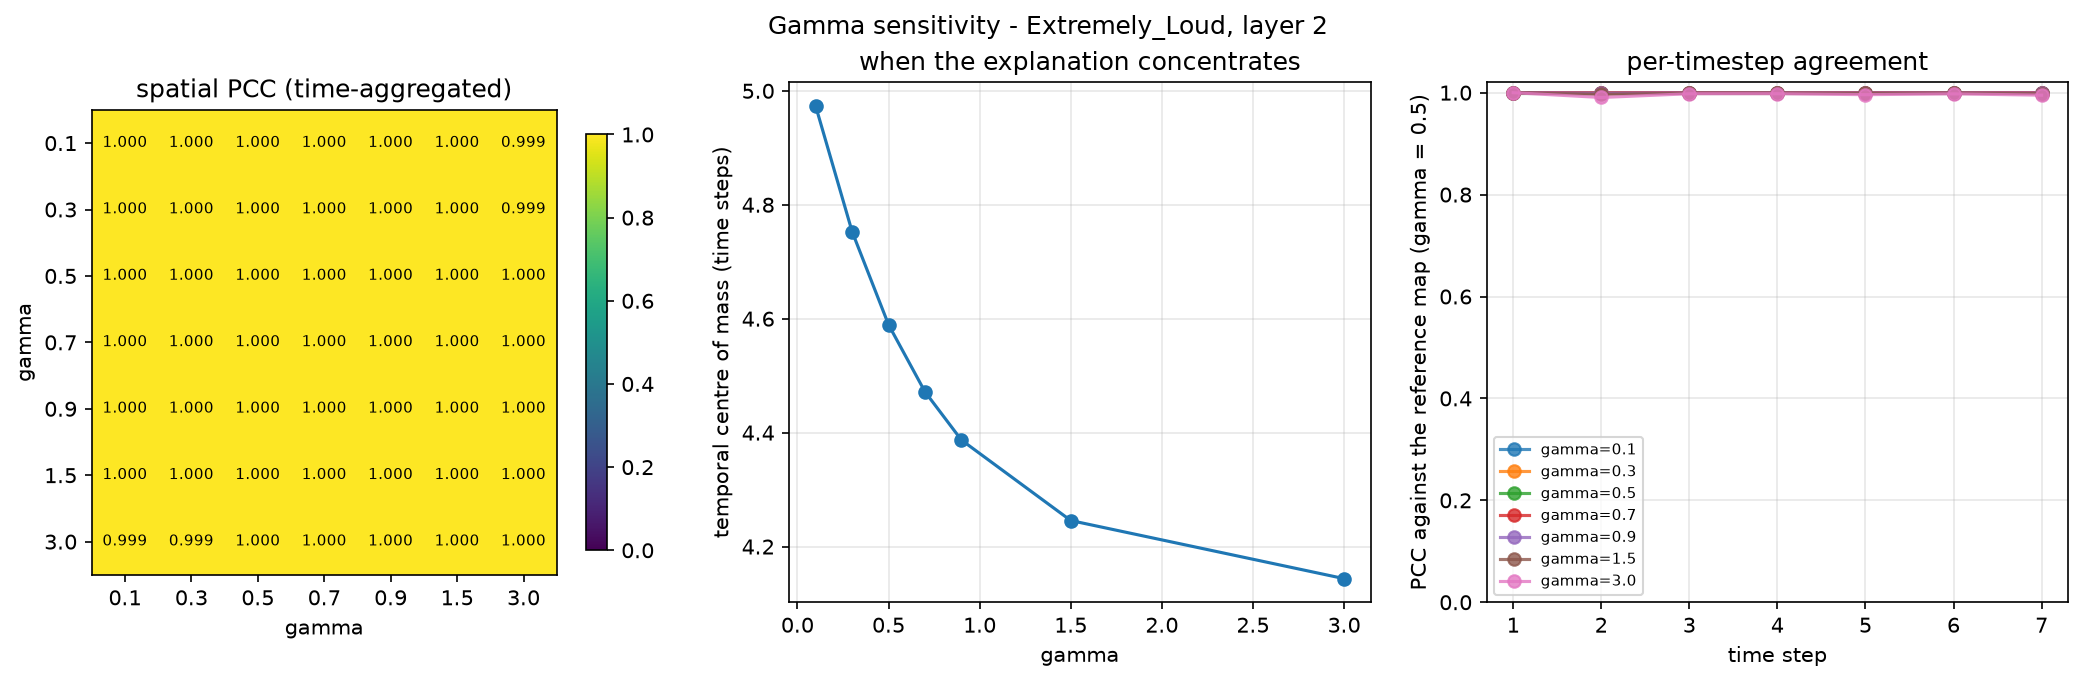
\includegraphics[width=\linewidth]{gamma_Extremely_Loud.png}\\[0.5em]
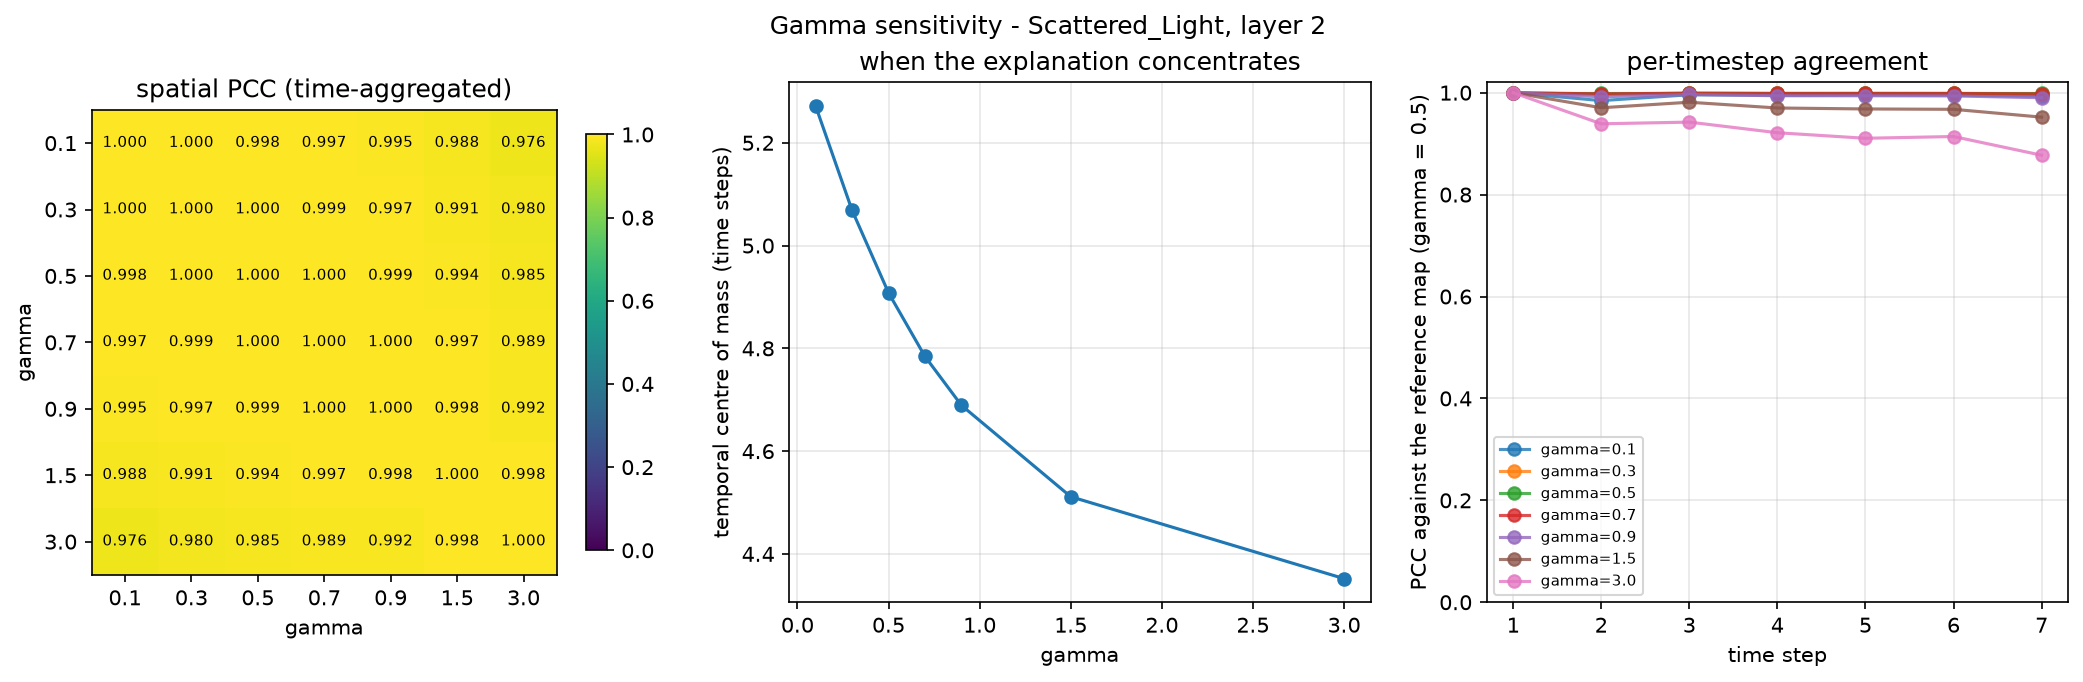
\includegraphics[width=\linewidth]{gamma_Scattered_Light.png}
\caption{$\gamma$ sensitivity at layer 2 for Blip, Extremely\_Loud and
Scattered\_Light, fifteen validation images per class (Violin\_Mode is in
Figure~\ref{fig:gamma}).}
\label{fig:gamma-others}
\end{figure}

\section{The quantization grid}

\begin{figure}[htbp]
\centering
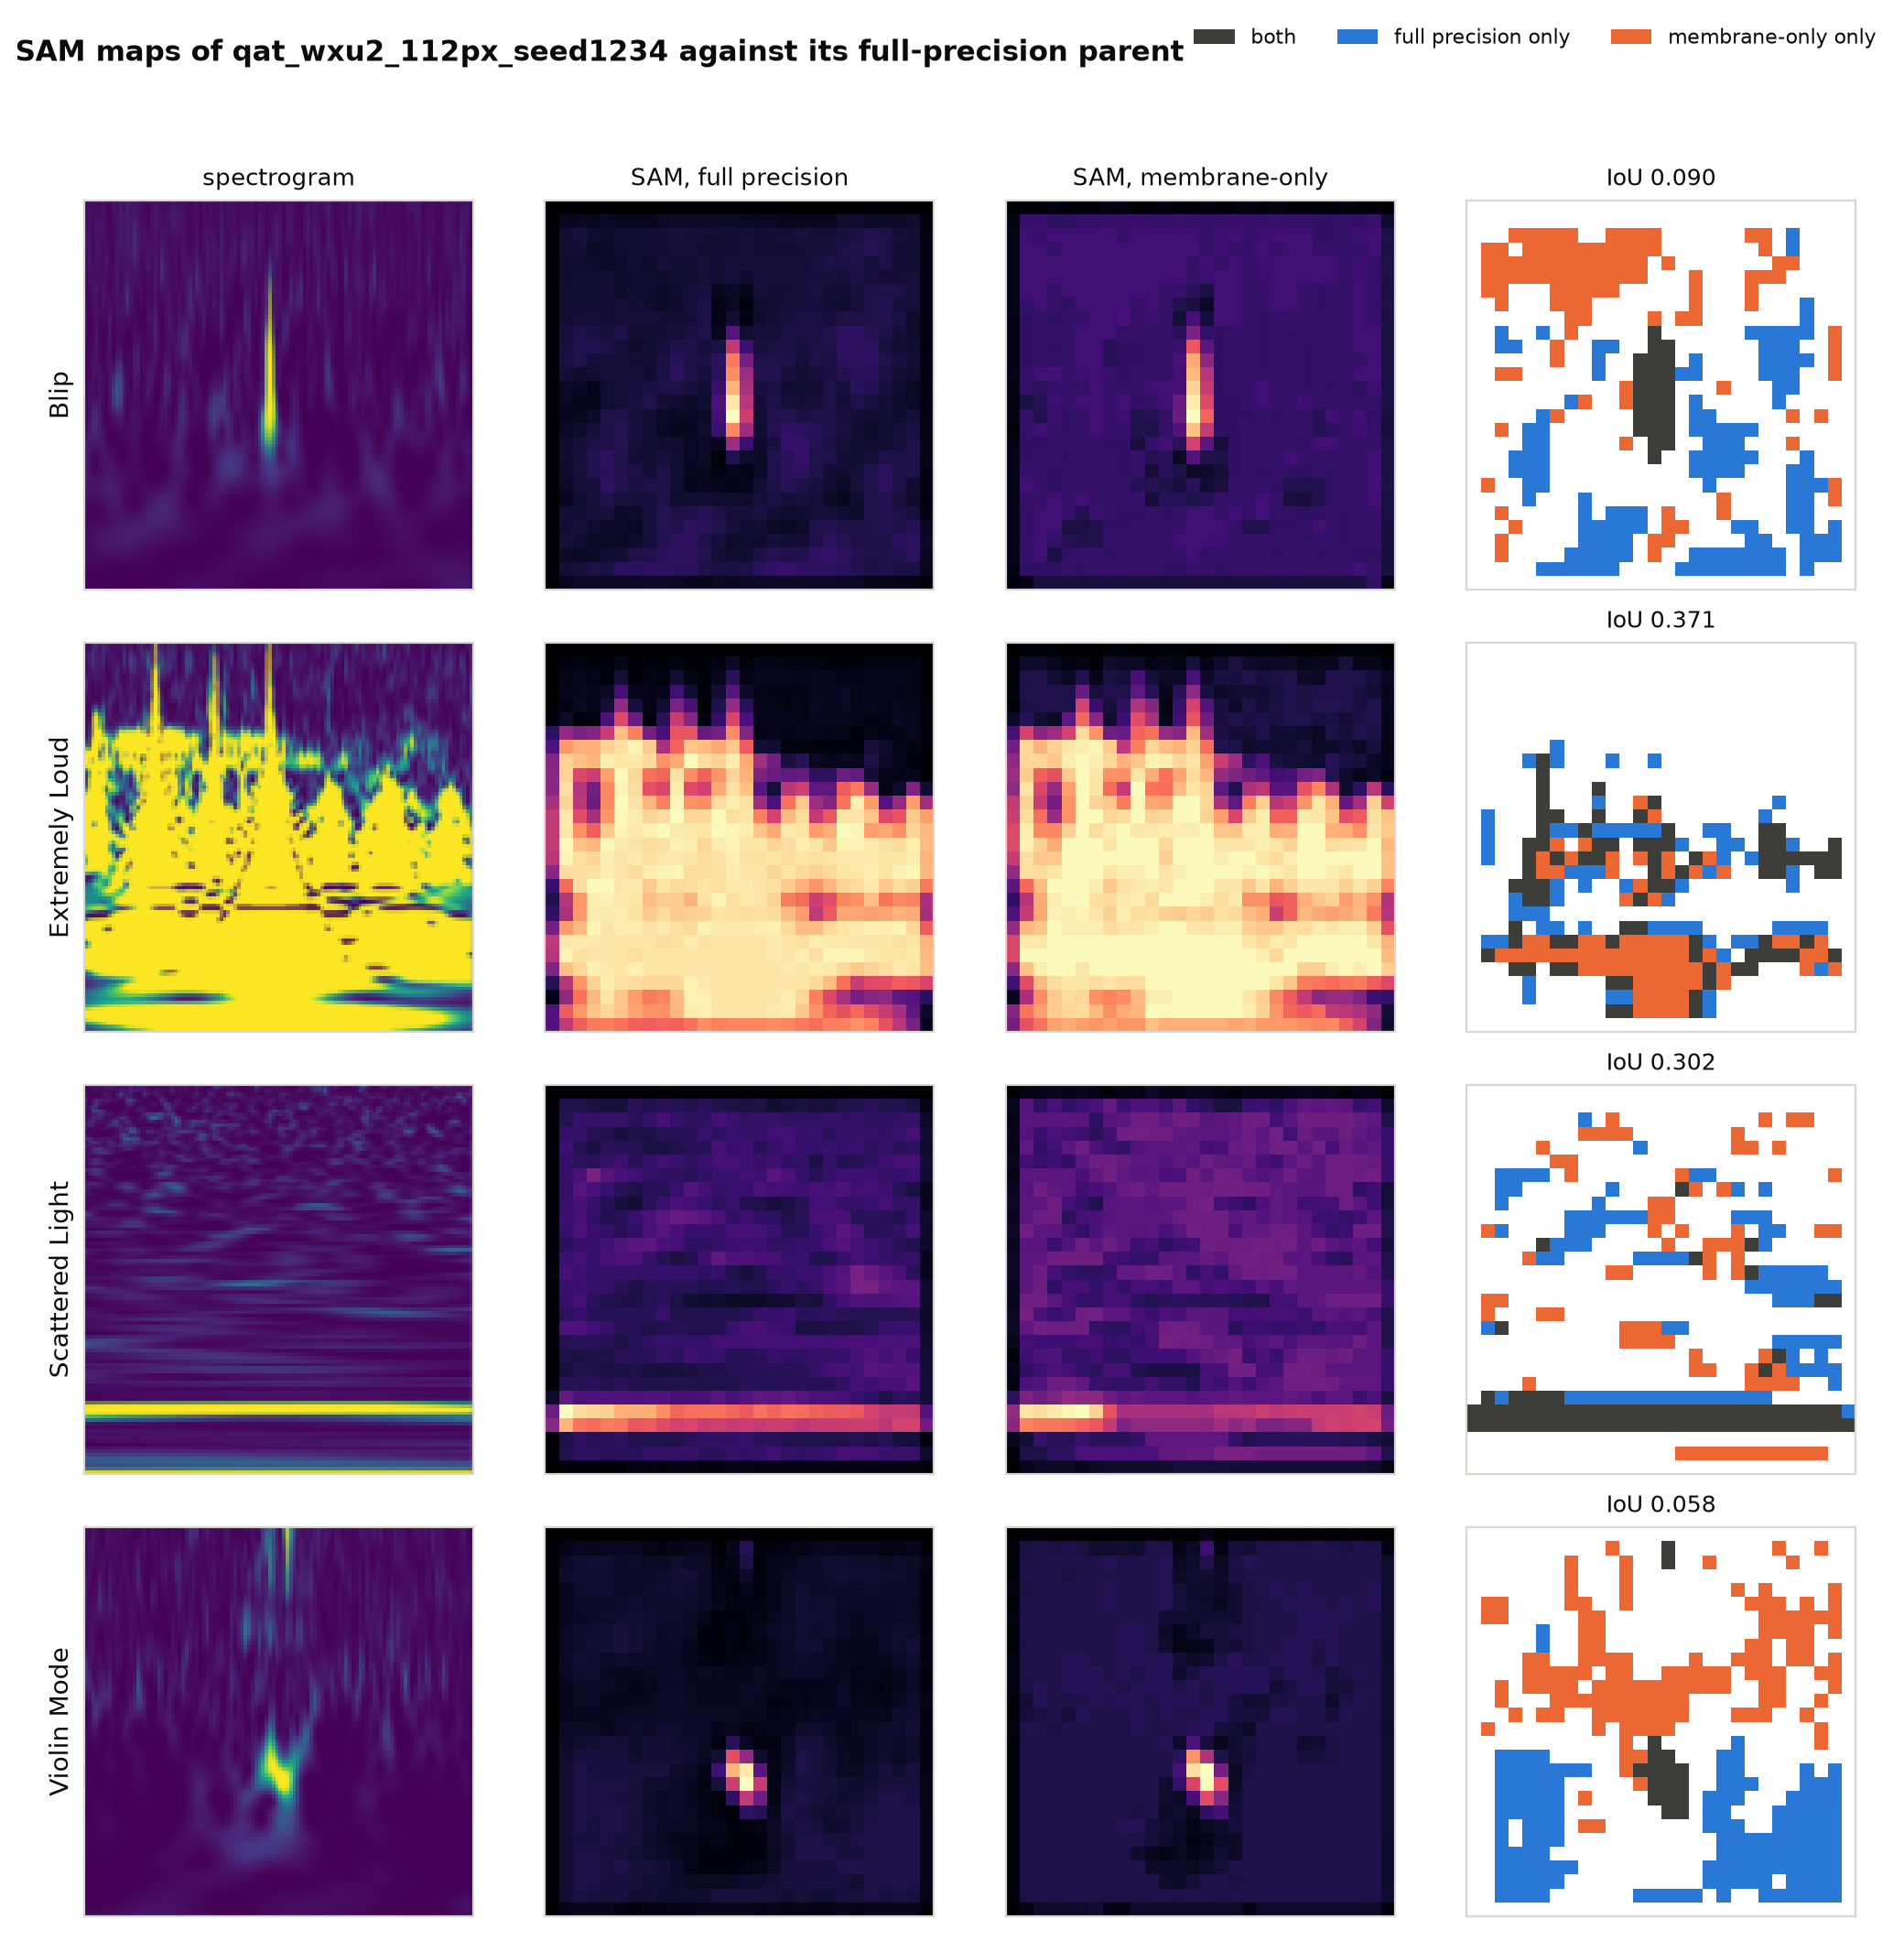
\includegraphics[width=\linewidth]{app_sam_comparison_seed1234.png}
\caption{As Figure~\ref{fig:sam-qat}, seed 1234, the seed with the lowest
overlap of the arm. In every row the highest-scoring positions coincide; the
disagreement lies in the lower-ranked positions that complete the 20\,\% set.}
\label{fig:app-sam-1234}
\end{figure}

\begin{figure}[htbp]
\centering
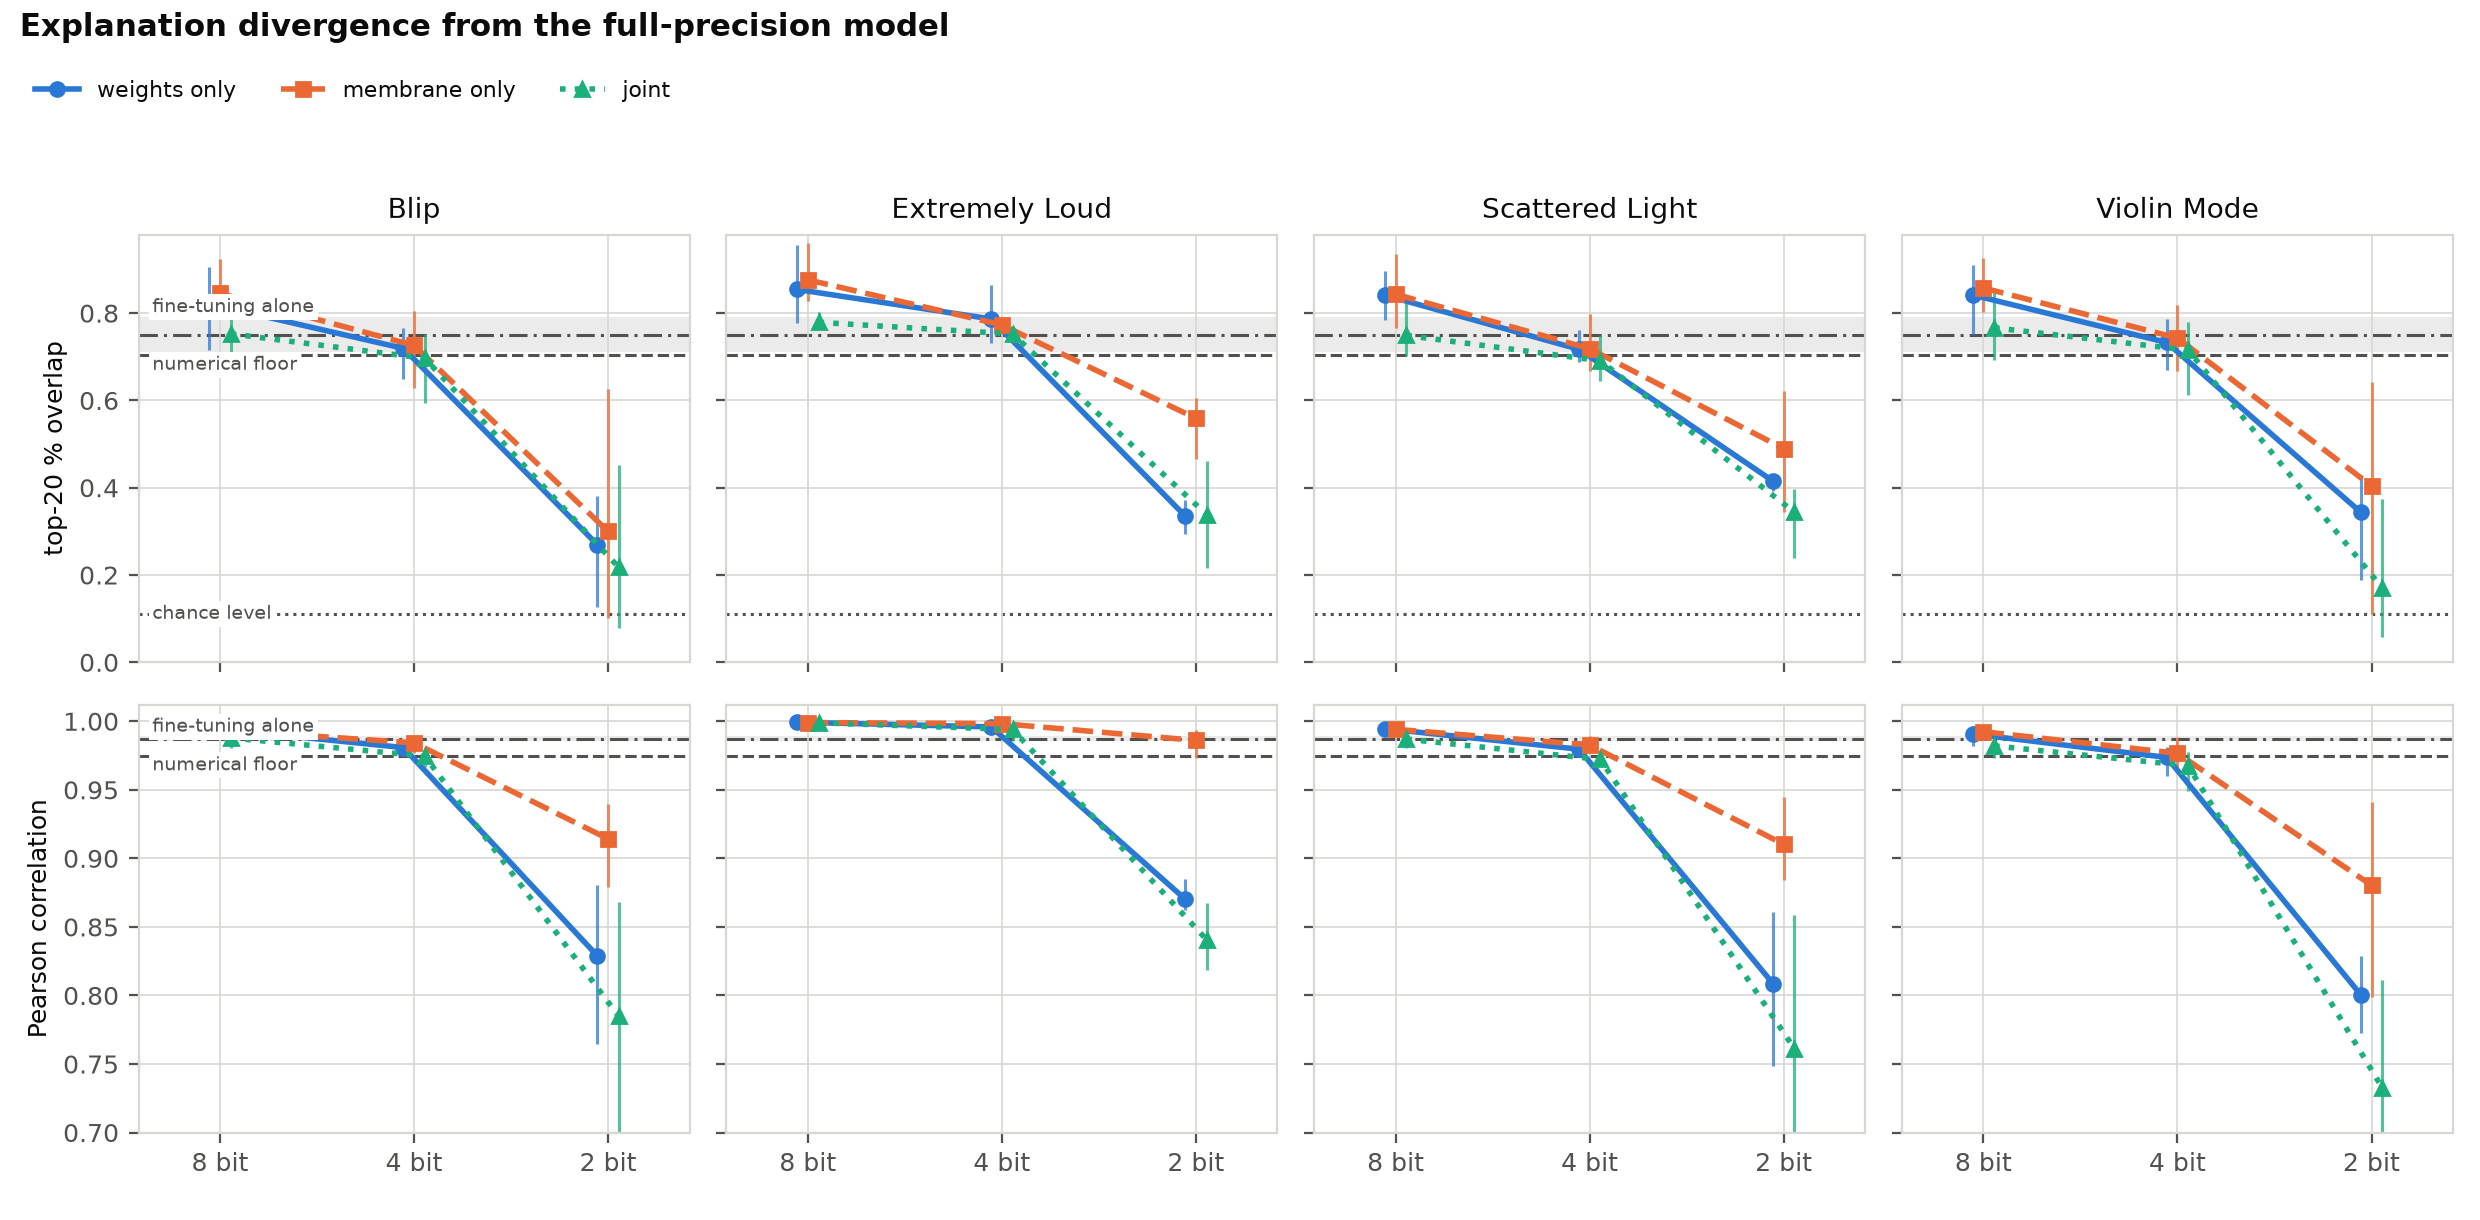
\includegraphics[width=\linewidth]{app_divergence_per_class.png}
\caption{Top-20\,\% IoU (top) and spatial PCC (bottom) per class against
bit-width, mean over three seeds, bars spanning the seeds. Dashed line: numerical
floor of the worst class; dash-dot line and grey band: fine-tuning level, mean
over classes and seeds and its seed range. The per-class levels against which the
grid is read are in Table~\ref{tab:levels-class}, the values in
Tables~\ref{tab:grid-iou} and~\ref{tab:grid-perclass}.}
\label{fig:app-divergence-class}
\end{figure}

\begin{figure}[htbp]
\centering
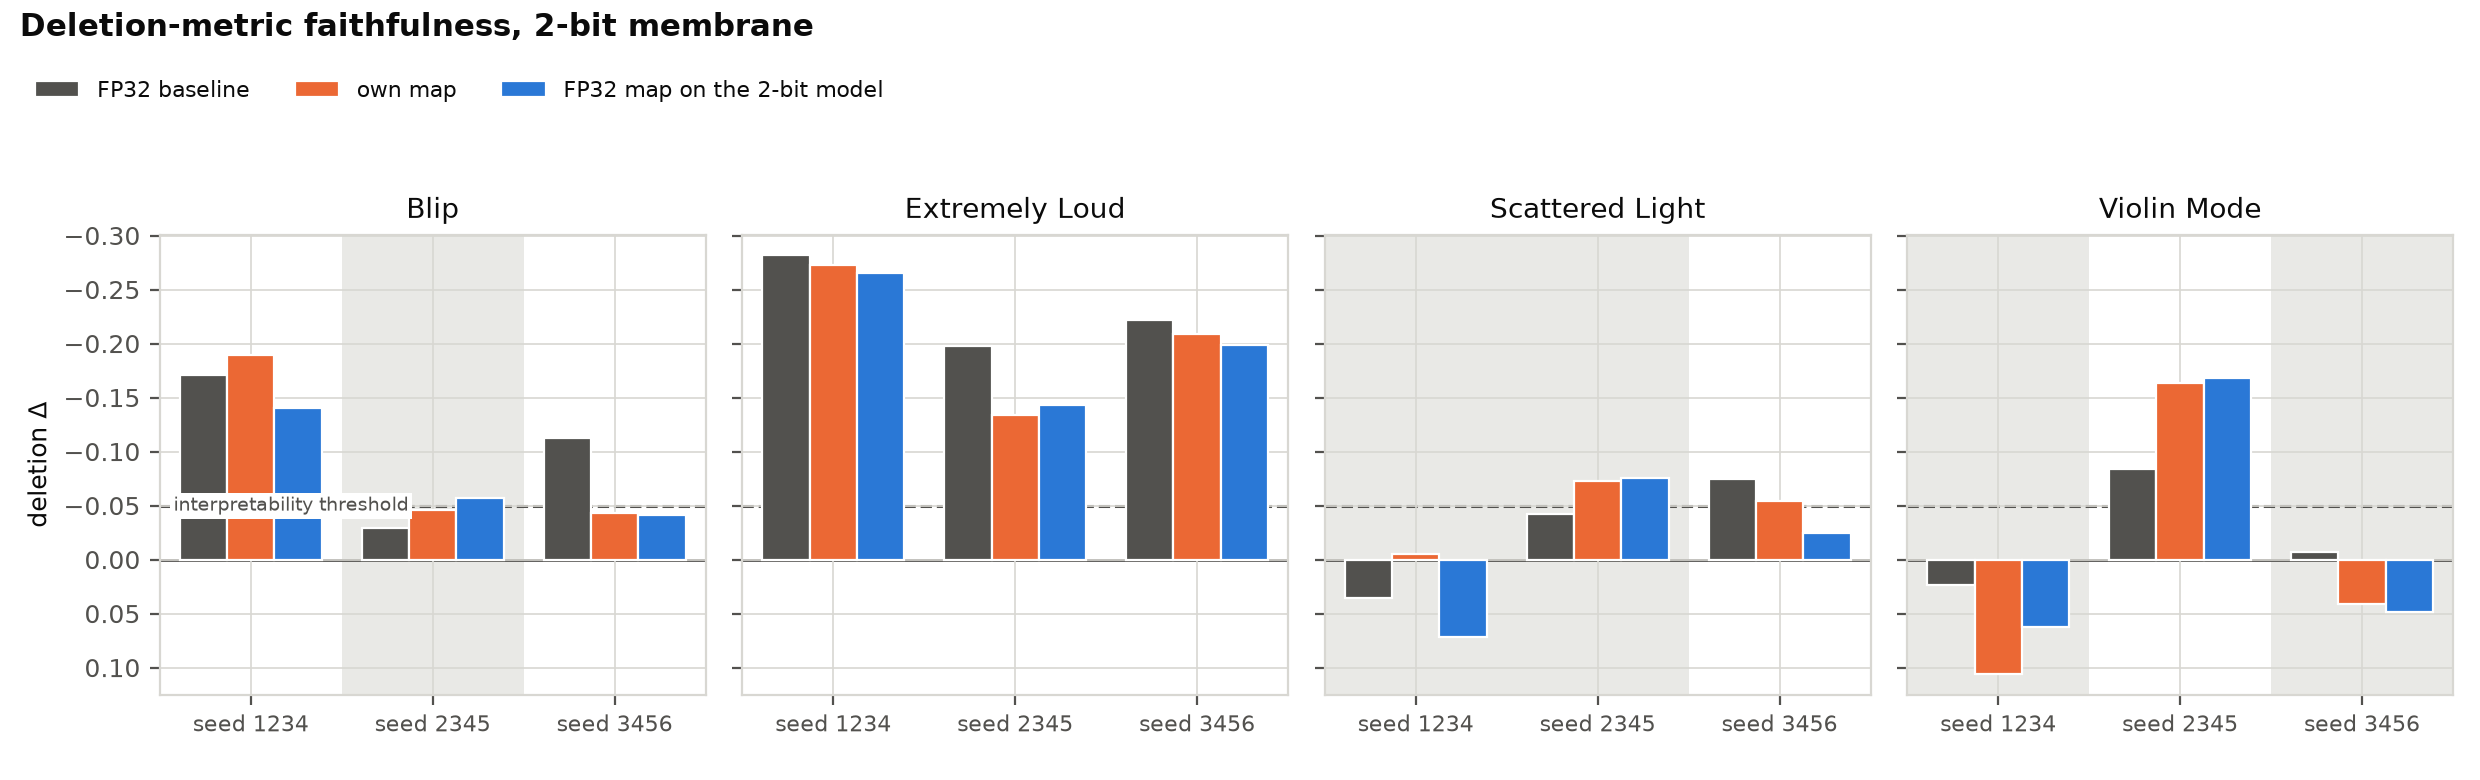
\includegraphics[width=\linewidth]{app_faithfulness_per_class.png}
\caption{Deletion gap $\Delta$ (inverted axis: upward is more faithful) of the
parent with its own map, of the 2-bit membrane model with its own map, and of the
2-bit membrane model with the parent's map, per class and seed, fifteen
validation images per cell. Shaded panels: the five cells whose parent baseline
does not reach the interpretability threshold of $0.05$ (dashed line), omitted
from Table~\ref{tab:cross-faith}.}
\label{fig:app-faithfulness}
\end{figure}

\begin{figure}[htbp]
\centering
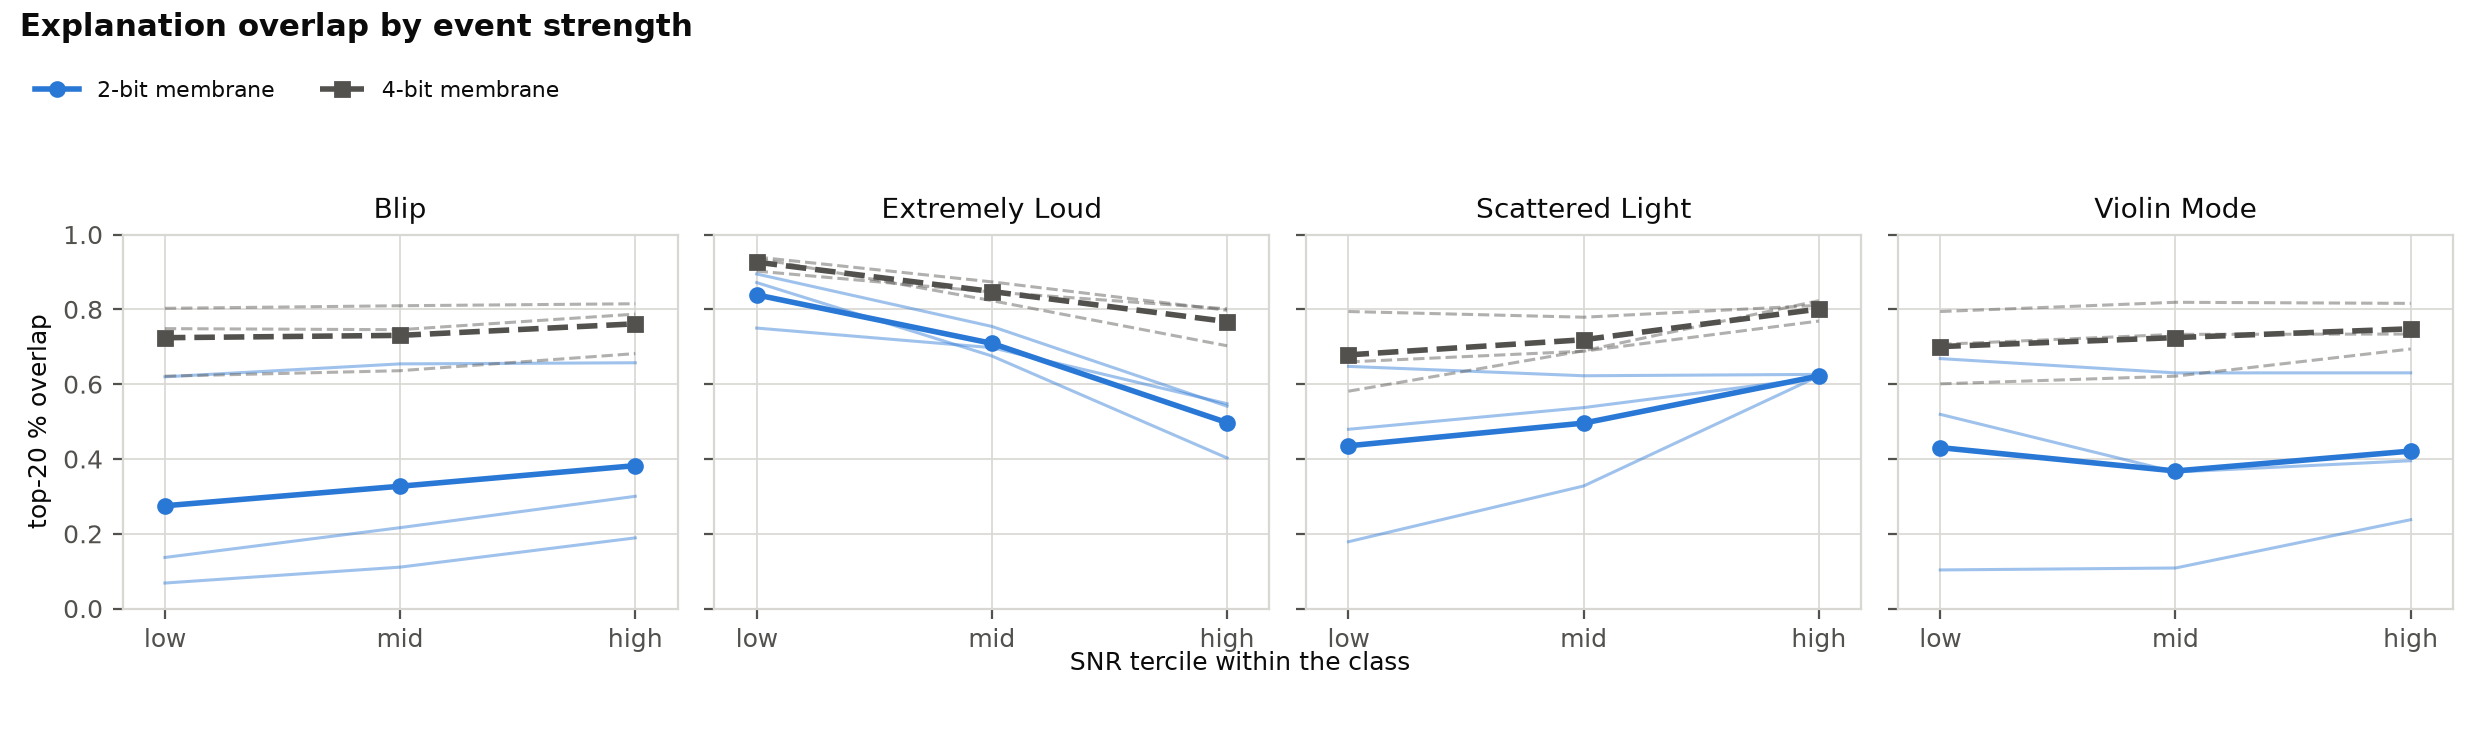
\includegraphics[width=\linewidth]{app_stratification_per_class.png}
\caption{Top-20\,\% IoU by SNR tercile computed within each class, membrane arm
at 2 and 4 bits; thick lines are the mean of the three seeds, thin lines single
seeds, fifteen images per cell. The gradients are those of
Table~\ref{tab:stratified}.}
\label{fig:app-stratification}
\end{figure}

\begin{figure}[htbp]
\centering
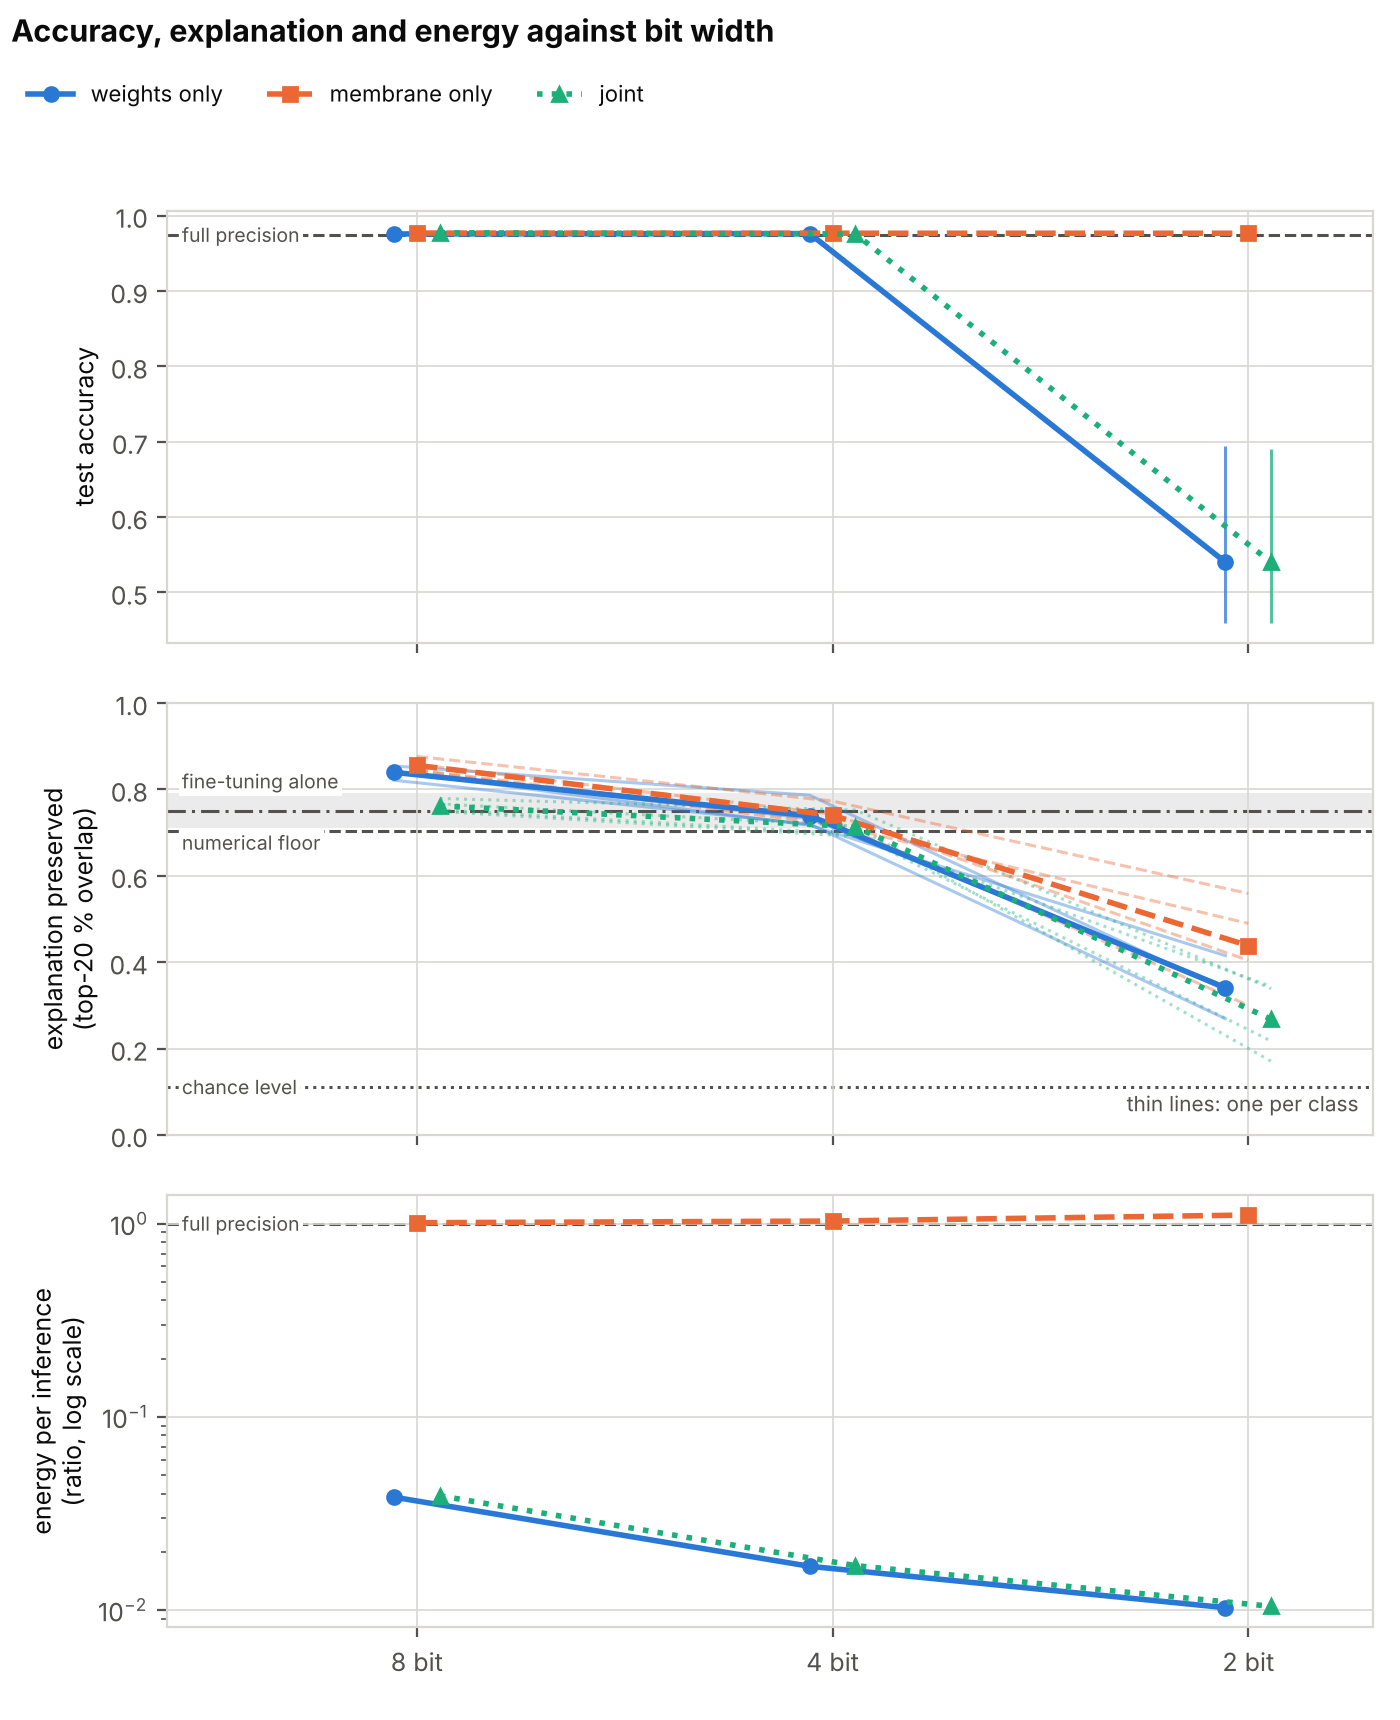
\includegraphics[width=0.8\linewidth]{app_summary_bits.png}
\caption{Test-set counterpart of Figure~\ref{fig:headline}: test accuracy (top),
top-20\,\% IoU measured on validation with one thin line per class (middle),
estimated energy relative to the parent (bottom), mean over three seeds.}
\label{fig:app-summary-test}
\end{figure}

%=======================================================================
\chapter{Algorithms}
\label{app:algorithms}

\makeatletter
\begingroup
\renewcommand*{\float@listhead}[1]{\section*{#1}}%
\addcontentsline{toc}{section}{List of Algorithms}
\listofalgorithms
\bigskip
\endgroup
\makeatother

{\raggedright
The procedures of Algorithms~\ref{alg:divergence}--\ref{alg:energy} are
implemented, in order, in \texttt{xai/divergence\_metrics.py},
\texttt{xai/perturbation\_floor.py}, \texttt{scripts/evaluate\_model.py} together
with \texttt{scripts/per\_image\_cv.py}, and \texttt{xai/energy.py}.
$\mathrm{SAM}$ denotes Algorithm~\ref{alg:sam}.\par}

\begin{algorithm}[htbp]
\caption{Explanation divergence between a quantized model and its parent}
\label{alg:divergence}
\begin{algorithmic}[1]
\REQUIRE parent $f_A$, quantized model $f_B$ of the same seed, images $X_c$
         (first 20 of class $c$ in loader order), layer $\ell = 2$,
         $\gamma = 0.5$, $k = 0.20$
\ENSURE  per-class PCC, IoU$_k$, signed and absolute CoM shift, per-step PCC
\FOR{$x \in X_c$}
  \STATE $M^{A} \gets \mathrm{SAM}(f_A, x, \ell, \gamma)$,\quad
         $M^{B} \gets \mathrm{SAM}(f_B, x, \ell, \gamma)$ \COMMENT{$[T, H, W]$}
  \STATE $A \gets \sum_t M^{A}_t$,\quad $B \gets \sum_t M^{B}_t$
  \STATE $\rho_x \gets \mathrm{PCC}(A, B)$ \COMMENT{undefined if either map is constant}
  \STATE $A_k \gets \{i : A_i > Q_{1-k}(A)\}$,\quad $B_k \gets \{i : B_i > Q_{1-k}(B)\}$
  \STATE $J_x \gets |A_k \cap B_k| \,/\, |A_k \cup B_k|$
  \STATE $\delta_x \gets \mathrm{CoM}(M^{B}) - \mathrm{CoM}(M^{A})$ \COMMENT{Eq.~\ref{eq:com}; $\delta_x < 0$: earlier}
  \FOR{$t = 1$ \TO $T-1$}
    \STATE $r_{x,t} \gets \mathrm{PCC}(M^{A}_t, M^{B}_t)$
  \ENDFOR
\ENDFOR
\RETURN means over $X_c$, ignoring undefined values, of $\rho_x$, $J_x$,
        $\delta_x$, $|\delta_x|$ and $r_{x,t}$
\end{algorithmic}
\end{algorithm}

\begin{algorithm}[htbp]
\caption{Numerical floor by weight perturbation}
\label{alg:floor}
\begin{algorithmic}[1]
\REQUIRE reference checkpoint $f$ (seed 1234), fractions
         $\Phi = \{0.01, 0.1, 0.5, 1\}$, noise seed 999, images $X_c$ (15 per class)
\ENSURE  per-class PCC, IoU$_k$, $|\Delta\mathrm{CoM}|$, per-step PCC at every fraction
\STATE $w_{\max} \gets \max |w|$ over all convolutional and linear weights
\STATE $s_8 \gets 2 w_{\max} / (2^{8} - 1)$ \COMMENT{global 8-bit step, $0.00168$}
\FOR{$\phi \in \Phi$}
  \STATE $\tilde f \gets$ copy of $f$; add $\mathcal{N}(0, (\phi s_8)^2)$ to every
         weight tensor \COMMENT{biases and LIF buffers untouched}
  \STATE compare $\tilde f$ with $f$ on $X_c$ as in Algorithm~\ref{alg:divergence}
\ENDFOR
\end{algorithmic}
\end{algorithm}

\begin{algorithm}[htbp]
\caption{Coefficient of variation of the inter-spike intervals}
\label{alg:cvisi}
\begin{algorithmic}[1]
\REQUIRE model $f$, validation partition $\mathcal{V}$, $T = 8$, 200 positions
         per layer, seed 42, minimum of 5 intervals
\ENSURE  pooled CV per layer and its defined fraction; per-image CV statistics
\STATE draw 200 neuron positions $P_\ell$ per hidden layer, once, at the first batch
\STATE $\mathcal{I}_p \gets \emptyset$ for every $p \in P_\ell$
\FOR{$x \in \mathcal{V}$}
  \STATE $S \gets$ hidden spike trains of $f(x)$
  \FOR{every hidden neuron $n$}
    \STATE $\tau \gets \{t : S_{n,t} = 1\}$,\quad $d \gets$ successive differences of $\tau$
    \IF{$n \in P_\ell$}
      \STATE $\mathcal{I}_n \gets \mathcal{I}_n \cup d$ \COMMENT{pooled over images}
    \ENDIF
    \IF{$|\tau| \geq 3$}
      \STATE $\mathrm{CV}_{n,x} \gets \sigma(d) / \mu(d)$ \COMMENT{per-image; two intervals at least}
    \ENDIF
  \ENDFOR
\ENDFOR
\STATE $\mathrm{CV}_p \gets \sigma(\mathcal{I}_p) / \mu(\mathcal{I}_p)$ for every
       $p$ with $|\mathcal{I}_p| \geq 5$
\RETURN per layer: mean of $\mathrm{CV}_p$, fraction of $P_\ell$ where it is
        defined; mean of $\mathrm{CV}_{n,x}$, fraction of neuron-image pairs
        with $|\tau| \geq 3$, fraction with $\mathrm{CV}_{n,x} = 0$
\end{algorithmic}
\end{algorithm}

\begin{algorithm}[htbp]
\caption{Energy and memory of one operating point}
\label{alg:energy}
\begin{algorithmic}[1]
\REQUIRE per-hidden-layer firing rates $f_1, \dots, f_4$ of the selected
         checkpoint, $T$, dense MAC counts $\mathrm{MAC}_\ell$, weight bit-width
         $b_w$, membrane bit-width $b_u$ (absent: 32-bit float), $N_w = 295\,088$
         weights, $N_u = 94\,080$ hidden neurons
\ENSURE  synaptic operations, energy, memory
\IF{$b_w$ absent}
  \STATE $c_{\mathrm{MAC}} \gets 4.6$\,pJ,\quad $c_{\mathrm{AC}} \gets 0.9$\,pJ
\ELSE
  \STATE $c_{\mathrm{AC}} \gets 0.03\,(b_w/8)$\,pJ,\quad
         $c_{\mathrm{MAC}} \gets 0.2\,(b_w/8)^2 + c_{\mathrm{AC}}$\,pJ
         \COMMENT{exact at 8 bits, extrapolated below}
\ENDIF
\STATE $E \gets \mathrm{MAC}_{\mathrm{conv1}} \cdot c_{\mathrm{MAC}}$
       \COMMENT{analog input, computed once}
\FOR{$(\ell, g) \in \{(\mathrm{conv2}, 1), (\mathrm{conv3}, 2), (\mathrm{conv4}, 3), (\mathrm{linear}, 4)\}$}
  \STATE $\mathrm{SOP}_\ell \gets f_g \cdot T \cdot \mathrm{MAC}_\ell$,\quad
         $E \gets E + \mathrm{SOP}_\ell \cdot c_{\mathrm{AC}}$
\ENDFOR
\STATE $\mathrm{Mem} \gets N_w \cdot (b_w \text{ or } 32)/8 + N_u \cdot (b_u \text{ or } 32)/8$ bytes
\RETURN $\sum_\ell \mathrm{SOP}_\ell$, $E$, $\mathrm{Mem}$
\end{algorithmic}
\end{algorithm}

%=======================================================================
\chapter{Reproducibility}
\label{app:reproducibility}

All code, configuration and result files are in the public repository
\begin{center}\url{https://github.com/devs-glitch/Tesi}\end{center}
Every analysis reads the model, the hyperparameters, the SAM layer and $\gamma$,
and the partition from \texttt{config/baseline\_manifest.json}.

\section{Environment and data}

The code requires Python $\geq 3.12$ and is installed from the repository root
with \texttt{pip install -e .} followed by \texttt{pip install -r
requirements.txt} (PyTorch $\geq 2.5$, torchvision $\geq 0.20$, snnTorch $\geq
0.9$, Optuna $\geq 4.0$, Weights \& Biases $\geq 0.18$, NumPy $\geq 2.0$,
pandas, scikit-learn, umap-learn, matplotlib, seaborn). Every script is run
from the repository root as a module, \texttt{python -m
<package>.<script>}. All training and evaluation ran on a single 6\,GB consumer
GPU; the thirty fine-tuning runs of the grid took $46\,924$\,s ($13.0$\,h).

The exact versions of every package used for the reported runs are recorded in
\texttt{requirements-lock.txt}; the runs used PyTorch 2.6, whose
\texttt{torch.clamp} passes a gradient of 1 at the ends of its range. More recent
versions (2.14 among them) pass 0 there, so the quantizer sets the gradient on
its grid explicitly, and \texttt{python -m model.quantization} checks it.

The metadata are the Gravity Spy release on Zenodo, record
5649212~\cite{glanzer2021}. The selected events are written to
\texttt{data/processed/selected\_dataset.csv} and the spectrograms to
\texttt{data/processed/<class>/}. The partition file
\texttt{data/split\_assignment.csv} lists $9\,568$ files; the two that are
unavailable at source are listed in \texttt{data/corrupted\_files.txt} and
dropped from the training partition at load time. The first sixteen hexadecimal
digits of its SHA-256 digest, \texttt{754b2515b6509075}, are recorded in the
manifest and checked by \texttt{scripts/verify\_manifest.py}.

\section{Seeds}

Partition: 42. Class balancing and UMAP subsample: 42. Training, reference and
fine-tuning: 1234, 2345, 3456. CV-ISI positions: 42. Weight perturbation of the
numerical floor: 999. Random deletion order: 42 for the reference deletion
metric, a seeded generator (seed 0) for cross-faithfulness. Image samples for
every SAM analysis are the first $n$ validation images of each class in loader
order, so they are identical across models.

\section{From result to script}

Tables~\ref{tab:repro-a} and~\ref{tab:repro-b} list the scripts in the order in
which they must be run. Trained checkpoints are written to
\texttt{runs/<tag>/} (\texttt{best\_model.pt}, \texttt{final\_model.pt},
\texttt{run.json}) and are not versioned; every step from the per-model
validation pass onwards needs them.

\begin{table}[htbp]
\centering
\footnotesize
\renewcommand{\_}{\textunderscore\allowbreak}%
\begin{tabular}{>{\raggedright\arraybackslash}p{0.26\linewidth}>{\raggedright\arraybackslash}p{0.33\linewidth}>{\raggedright\arraybackslash}p{0.31\linewidth}}
\toprule
Result & Module & Output \\
\midrule
Metadata download & \texttt{scripts.dataset\_downloader} & raw CSV files \\
Class and feature selection, balancing & \texttt{scripts.data\_prep} &
  \texttt{data/processed/selected\_dataset.csv}, Figs.~\ref{fig:label-counts}--\ref{fig:umap} \\
Spectrogram download & \texttt{scripts.image\_downloader} & \texttt{data/processed/<class>/} \\
Frozen partition & \texttt{scripts.freeze\_split} & \texttt{data/split\_assignment.csv} \\
Tabular baseline & \texttt{scripts.tabular\_baseline} & \texttt{results/tabular\_baseline.json} \\
Resolution study & \texttt{scripts.resolution\_study} & \texttt{runs/resolution\_study.csv}, copied to \texttt{results/} \\
Dead neurons by resolution & \texttt{scripts.dead\_neurons\_by\_resolution --out results/dead\_neurons.json} & \texttt{results/dead\_neurons.json} \\Hyperparameter search (v4, v5) & \texttt{scripts.tune} & \texttt{config/best\_hyperparams*.json} \\
FP32 reference, manifest & \texttt{scripts.fp32\_reference} & \texttt{config/baseline\_manifest.json} \\
Cutoff sweep & \texttt{scripts.dead\_neuron\_cutoff\_sweep} & \texttt{results/tables/dead\_neuron\_sweep.csv}, Fig.~\ref{fig:sweep} \\
Confusion matrix, firing rates, CV-ISI & \texttt{scripts.diagnostics\_figures} &
  Figs.~\ref{fig:confusion}, \ref{fig:firing}, \ref{fig:cvisi} \\
SAM per time step & \texttt{scripts.sam\_visualization} & Fig.~\ref{fig:sam-steps} \\
SAM class and layer statistics & \texttt{xai.sam\_class\_comparison}, \texttt{xai.sam\_layer\_comparison} &
  Figs.~\ref{fig:sam-class}, \ref{fig:sam-layers} \\
$\gamma$ sensitivity & \texttt{xai.gamma\_sensitivity\_analysis} & \texttt{results/gamma\_sensitivity.json}, Figs.~\ref{fig:gamma}, \ref{fig:gamma-others} \\
Deletion metric & \texttt{xai.deletion\_metric} & Table~\ref{tab:deletion}, Fig.~\ref{fig:deletion} \\
Independent solutions & \texttt{xai.noise\_floor} & \texttt{results/noise\_floor.json} \\
Numerical floor & \texttt{xai.perturbation\_floor} & \texttt{results/perturbation\_floor.json} \\
\bottomrule
\end{tabular}
\caption{Reproducibility, full-precision stages. Steps up to the resolution
study read the input size from the environment variable
\texttt{SNN\_INPUT\_SIZE}; from the reference onwards it is read from the
manifest.}
\label{tab:repro-a}
\end{table}

\begin{table}[htbp]
\centering
\footnotesize
\renewcommand{\_}{\textunderscore\allowbreak}%
\begin{tabular}{>{\raggedright\arraybackslash}p{0.26\linewidth}>{\raggedright\arraybackslash}p{0.33\linewidth}>{\raggedright\arraybackslash}p{0.31\linewidth}}
\toprule
Result & Module & Output \\
\midrule
Membrane range & \texttt{scripts.membrane\_range} & \texttt{config/membrane.json} \\
Clipping study & \texttt{scripts.test\_clipping} & \texttt{results/clipping\_test.json} \\
Quantizers & \texttt{model.quantization} & --- \\
PTQ gate & \texttt{scripts.ptq\_check} & \texttt{results/ptq\_check.json} \\
Fine-tuning grid & \texttt{scripts.grid\_runner} (calls \texttt{scripts.train\_quantised}) &
  \texttt{runs/qat\_*}, \texttt{results/grid\_summary.json} \\
Per-model validation pass & \texttt{scripts.evaluate\_model} &
  \texttt{results/grid/<tag>.json}, \texttt{\_per\_sample.csv}, \texttt{\_rates.npz} \\
Fine-tuning level & \texttt{scripts.finetuning\_anchor} & \texttt{results/finetuning\_anchor.json} \\
SAM divergence & \texttt{xai.divergence\_metrics} & \texttt{results/divergence.json} \\
Cross-faithfulness & \texttt{xai.cross\_faithfulness} & \texttt{results/cross\_faithfulness.json} \\
SNR stratification & \texttt{xai.stratify} & \texttt{results/stratified.json} \\
EMD, disagreement subset & \texttt{scripts.grid\_analysis} & \texttt{results/grid\_analysis.json} \\
Per-image CV-ISI & \texttt{scripts.per\_image\_cv} & \texttt{results/per\_image\_cv.json} \\
Energy and memory & \texttt{xai.energy} & \texttt{results/energy.json} \\
Energy against the control & \texttt{xai.energy --rates final --baseline
  qat\_wxux\_\{input\_size\}px\_seed\{seed\} --out results/energy\_final.json} &
  \texttt{results/energy\_final.json} \\
SAM maps after quantization & \texttt{xai.sam\_qat\_comparison --run <tag>} &
  Figs.~\ref{fig:sam-qat}, \ref{fig:topk-sweep}, \ref{fig:app-sam-1234} \\
Grid figures and tables & \texttt{scripts.figures.result\_figures} &
  \texttt{results/tables/*.csv}, Figs.~\ref{fig:spike-stats}, \ref{fig:behaviour}, \ref{fig:app-divergence-class}--\ref{fig:app-summary-test} \\
Methods figures & \texttt{scripts.architecture\_figure}, \texttt{scripts.figures.*} &
  Figs.~\ref{fig:architecture}, \ref{fig:arms}, \ref{fig:scale-granularity}, \ref{fig:membrane-grid} \\
Grid summary figure & \texttt{scripts.figures.grid\_headline\_figure} & Fig.~\ref{fig:headline} \\
Test set (opened once) & \texttt{scripts.evaluate\_test} &
  \texttt{results/test/}, \texttt{results/test\_opened.json} \\
\bottomrule
\end{tabular}
\caption{Reproducibility, quantization study. The test partition was opened
once, on 7 October 2026, for all thirty-three models; the opening is logged in
\texttt{results/test\_opened.json} and the script refuses a second one unless
forced.}
\label{tab:repro-b}
\end{table}